\documentclass[11pt,a4paper]{article}
\usepackage[utf8]{inputenc}
\usepackage{amsmath,amsfonts,amssymb}
\usepackage{geometry}
\geometry{top=1in,bottom=1in,left=1in,right=1in}
\usepackage{graphicx}
\usepackage{listings}
\usepackage{booktabs}
\usepackage{hyperref}
\usepackage{tikz}
\usetikzlibrary{shapes,arrows,positioning,calc}
\usepackage{xcolor}
\usepackage{microtype}
\usepackage{fancyhdr}

\hypersetup{
    colorlinks=true,
    linkcolor=blue,
    filecolor=magenta,      
    urlcolor=cyan,
    pdftitle={Autonomous Financial Agent Technical Documentation},
    pdfpagemode=FullScreen,
}

\definecolor{codegreen}{rgb}{0,0.6,0}
\definecolor{codegray}{rgb}{0.5,0.5,0.5}
\definecolor{codepurple}{rgb}{0.58,0,0.82}
\definecolor{backcolour}{rgb}{0.95,0.95,0.92}

\lstdefinestyle{mystyle}{
    backgroundcolor=\color{backcolour},   
    commentstyle=\color{codegreen},
    keywordstyle=\color{blue}\bfseries,
    numberstyle=\tiny\color{codegray},
    stringstyle=\color{codepurple},
    basicstyle=\ttfamily\footnotesize,
    breakatwhitespace=false,         
    breaklines=true,                 
    captionpos=b,                    
    keepspaces=true,                 
    numbers=left,                    
    numbersep=5pt,                  
    showspaces=false,                
    showstringspaces=false,
    showtabs=false,                  
    tabsize=2,
    frame=single,
    rulecolor=\color{codegray}
}
\lstset{style=mystyle}

\pagestyle{fancy}
\fancyhf{}
\rhead{\small{Autonomous Financial Agent}}
\lhead{\small{Technical Documentation}}
\rfoot{Page \thepage}

\title{\textbf{Autonomous Financial Agent}\\Architectural and Technical System Documentation}
\author{\textbf{Technical Development Team}}
\date{June 2026}

\begin{document}

\maketitle

\begin{abstract}
This document provides a comprehensive technical overview of the Autonomous Financial Agent, a privacy-first, multi-agent financial management application. The system ingests PDF bank statements, scrubs sensitive Personal Identifiable Information (PII) locally, parses and categorizes financial transactions, and facilitates natural language interactions. By leveraging advanced query routing, a text-to-SQL database agent, and an Indian Income Tax Advisory agent, the application allows users to query spending patterns deterministically and optimize their tax liabilities securely.
\end{abstract}

\tableofcontents
\newpage

\section{Introduction}
Managing personal and business finances is a major challenge for individuals, freelancers, and businesses. Standard financial applications often require users to manually input details or upload statements to servers, raising significant privacy concerns. Furthermore, extracting structured data from diverse PDF bank statements remains a tedious process.

The \textbf{Autonomous Financial Agent} addresses these challenges by offering:
\begin{itemize}
    \item \textbf{Privacy-First Uploads:} All uploaded statements undergo local, regex-based PII scrubbing before any external API or LLM processing, removing names, emails, card numbers, account numbers, and Indian tax identifiers (PAN and Aadhar).
    \item \textbf{High-Fidelity PDF Parsing:} Extraction of text and complex tables using cloud-based \texttt{LlamaParse} with a local fallback using \texttt{pdfplumber}.
    \item \textbf{Deterministic SQL Queries:} Users interact with their structured transaction records using natural language. A text-to-SQL translation agent converts these queries to read-only SQL SELECT queries with robust security controls.
    \item \textbf{Indian Income Tax Advisory:} Matches historical transactions with tax codes (such as Sections 80C, 80D, 44ADA, 80GG, and 80TTA of the Indian Income Tax Act) using Retrieval-Augmented Generation (RAG) and keyword analysis, recommending specific tax-saving strategies.
\end{itemize}

\section{System Architecture}
The application is structured as a three-tier system:
\begin{enumerate}
    \item \textbf{Frontend Dashboard:} Built using Next.js (React), TailwindCSS, and lucide icons. It provides a visual chat terminal, file upload utility, historical transaction listing, and tax advisory panels.
    \item \textbf{Backend REST API:} Developed using FastAPI, SQLAlchemy, and LangGraph. It contains routing logic, text processors, database models, and LLM integrations (OpenAI / Google Gemini).
    \item \textbf{Relational Database:} Supports a local SQLite database for rapid local development and testing, with a production option to connect to PostgreSQL (e.g., Supabase, AWS RDS).
\end{enumerate}

\subsection{Architecture Diagram}
Figure~\ref{fig:architecture} illustrates the layout and flow of data in the system.

\begin{figure}[htbp]
\centering
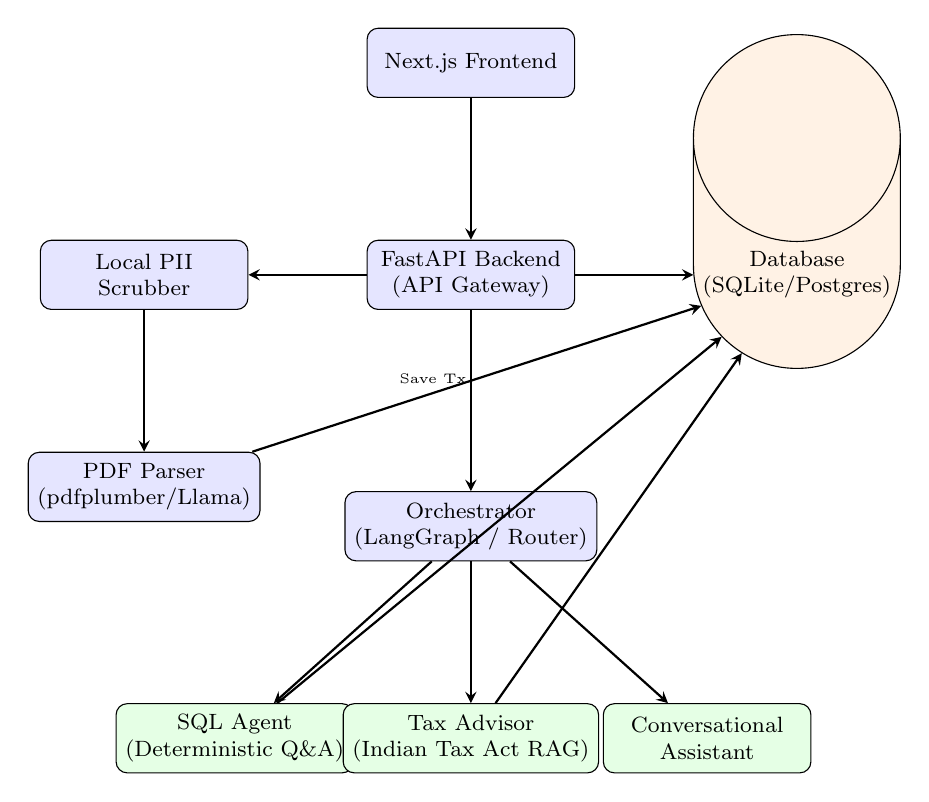
\begin{tikzpicture}[
    node distance=1.8cm and 1.5cm,
    block/.style={draw, fill=blue!10, rectangle, minimum height=2.5em, minimum width=7.5em, rounded corners, align=center, font=\footnotesize},
    agent/.style={draw, fill=green!10, rectangle, minimum height=2.5em, minimum width=7.5em, rounded corners, align=center, font=\footnotesize},
    db/.style={draw, fill=orange!10, cylinder, shape border rotate=90, minimum height=2.5em, minimum width=6em, align=center, font=\footnotesize},
    cloud/.style={draw, fill=red!10, ellipse, minimum height=2.5em, minimum width=7.5em, align=center, font=\footnotesize},
    arrow/.style={thick,->,>=stealth}
]
    % Draw nodes
    \node (user) [block] {Next.js Frontend};
    \node (fastapi) [block, below=of user] {FastAPI Backend\\(API Gateway)};
    \node (scrub) [block, left=of fastapi] {Local PII\\Scrubber};
    \node (parser) [block, below=of scrub] {PDF Parser\\(pdfplumber/Llama)};
    \node (db) [db, right=of fastapi] {Database\\(SQLite/Postgres)};
    
    \node (orchestrator) [block, below=of fastapi, yshift=-0.5cm] {Orchestrator\\(LangGraph / Router)};
    \node (sqlagent) [agent, below=of orchestrator, xshift=-3cm] {SQL Agent\\(Deterministic Q\&A)};
    \node (taxadvisor) [agent, below=of orchestrator] {Tax Advisor\\(Indian Tax Act RAG)};
    \node (chatnode) [agent, below=of orchestrator, xshift=3cm] {Conversational\\Assistant};

    % Draw connections
    \draw [arrow] (user) -- (fastapi);
    \draw [arrow] (fastapi) -- (scrub);
    \draw [arrow] (scrub) -- (parser);
    \draw [arrow] (parser) -- node[left, font=\tiny] {Save Tx} (db);
    \draw [arrow] (fastapi) -- (orchestrator);
    \draw [arrow] (orchestrator) -- (sqlagent);
    \draw [arrow] (orchestrator) -- (taxadvisor);
    \draw [arrow] (orchestrator) -- (chatnode);
    
    \draw [arrow] (sqlagent) -- (db);
    \draw [arrow] (taxadvisor) -- (db);
    \draw [arrow] (fastapi) -- (db);
    
\end{tikzpicture}
\caption{System Architecture and Transaction Flow}
\label{fig:architecture}
\end{figure}

\section{Database and Data Schema}
The storage layer holds user transactions and enforces separation of data by including a \texttt{user\_id} constraint on every record. The backend uses SQLAlchemy to declare database tables and model interactions.

\subsection{Database Schema Model}
The main storage structure is defined by the \texttt{transactions} table, which stores information parsed from bank statements. 

\begin{lstlisting}[language=Python, caption=SQLAlchemy Transaction Model (database.py)]
class DBTransaction(Base):
    __tablename__ = "transactions"

    id = Column(Integer, primary_key=True, index=True)
    user_id = Column(String, index=True)
    transaction_date = Column(Date, nullable=False)
    description = Column(String, nullable=False)
    amount = Column(Float, nullable=False)
    transaction_type = Column(String, nullable=False)  # DEBIT or CREDIT
    category = Column(String, nullable=False)
    notes = Column(Text, nullable=True)
\end{lstlisting}

Table~\ref{tab:schema} lists the fields of the \texttt{transactions} database schema in detail.

\begin{table}[htbp]
\centering
\begin{tabular}{llll}
\toprule
\textbf{Column Name} & \textbf{Data Type} & \textbf{Constraints} & \textbf{Description} \\
\midrule
\texttt{id} & INTEGER & Primary Key, Index & Unique identifier for the transaction record \\
\texttt{user\_id} & VARCHAR & Indexed & Identifies the user to isolate multi-tenant data \\
\texttt{transaction\_date} & DATE & NOT NULL & The transaction execution date (YYYY-MM-DD) \\
\texttt{description} & VARCHAR & NOT NULL & Transaction text memo / description \\
\texttt{amount} & FLOAT & NOT NULL & The monetary value of the transaction \\
\texttt{transaction\_type} & VARCHAR & NOT NULL & Either \texttt{DEBIT} (expense) or \texttt{CREDIT} (income) \\
\texttt{category} & VARCHAR & NOT NULL & Enum: FOOD, UTILITIES, RENT, TRAVEL, etc. \\
\texttt{notes} & TEXT & NULLABLE & Optional comments or tax-related flags \\
\bottomrule
\end{tabular}
\caption{Database Columns and Type Information}
\label{tab:schema}
\end{table}

\subsection{Query Sanitization and Security}
When running arbitrary queries dynamically generated by natural language processors, standard applications are prone to SQL injection attacks or destructive operations (e.g., drops, updates, deletes). The Autonomous Financial Agent mitigates these security threats in two ways:
\begin{enumerate}
    \item \textbf{Destructive Keyword Filter:} Before passing the generated SQL to the connection manager, the backend checks the text against a list of blocked keywords: \texttt{DROP}, \texttt{DELETE}, \texttt{UPDATE}, \texttt{INSERT}, \texttt{ALTER}, \texttt{CREATE}, \texttt{TRUNCATE}, \texttt{RENAME}, \texttt{GRANT}, \texttt{REVOKE}. If any blocklist term is found matching a word boundary, an exception is thrown.
    \item \textbf{Parameter Binding:} The query requires isolation by user, which is enforced programmatically by forcing the parameter binding \texttt{:user\_id} in the database query.
\end{enumerate}

\section{Data Processing Pipeline}
When a statement is uploaded, it runs through a sequential pipeline consisting of parsing, scrubbing, categorization, and storage.

\subsection{PDF Statement Parsing}
The statement parsing engine (\texttt{parsing.py}) loads the document. If an API key for \texttt{LlamaParse} is present in the environment variables, the engine delegates parsing to the LlamaIndex LlamaParse service. This uses optical character recognition (OCR) and layout modeling to parse structured transaction tables into a clean markdown format.

If \texttt{LlamaParse} is absent or encounters network issues, the pipeline falls back to \texttt{pdfplumber}. This local Python utility extracts text coordinates and reconstructs tables page-by-page, formatting columns using Markdown table syntax (\texttt{| Column 1 | Column 2 |}).

\subsection{Personal Identifiable Information (PII) Scrubbing}
Privacy is maintained by ensuring that all financial statement text passes through the local PII Scrubber before any LLM processing. This is critical when utilizing public LLMs, as statements frequently contain names, phone numbers, addresses, account details, and tax identifiers.

The PII scrubber uses compiled regular expressions to match and mask data:
\begin{itemize}
    \item \textbf{Email Addresses:} Matches standard RFC 5322 structures and replaces them with \texttt{[EMAIL]}.
    \item \textbf{Credit Card Numbers:} Matches 13 to 16 digit numbers (spaced or hypenated) and replaces them with \texttt{[CARD\_NUMBER]}.
    \item \textbf{Indian PAN Cards:} Matches the standard regex format \texttt{\textbackslash b[A-Z]\{5\}[0-9]\{4\}[A-Z]\textbackslash b} and replaces it with \texttt{[PAN\_NUMBER]}.
    \item \textbf{Indian Aadhar Cards:} Matches standard 12-digit spaced sequences and replaces them with \texttt{[AADHAR\_NUMBER]}.
    \item \textbf{Bank Account Numbers:} Replaces sequences of 9 to 18 digits (excluding standard currency amounts) with \texttt{[ACCOUNT\_NUMBER]}.
    \item \textbf{Phone Numbers:} Replaces international and standard Indian ten-digit telephone strings with \texttt{[PHONE]}.
    \item \textbf{Customer Names:} Replaces personal names found adjacent to header metadata labels (e.g., \textit{``Name:''}, \textit{``Dear Mr.''}) with \texttt{[CUSTOMER\_NAME]}.
\end{itemize}

\subsection{Transaction Categorization}
Categorization assigns a label to each transaction. The backend handles this in two ways:
\begin{enumerate}
    \item \textbf{LLM Structured Output (Preferred):} Uses the Pydantic-based structured output features in OpenAI (\texttt{gpt-4o-mini}) or Gemini (\texttt{gemini-1.5-flash}) to extract transaction objects matching a strict JSON schema. This handles natural language descriptions and categorizes transactions into predefined categories.
    \item \textbf{Local Heuristic Classifier (Fallback):} Uses regex patterns and keyword dictionaries to process statement lines locally. Keywords map descriptions to target categories (e.g., \textit{Uber, Ola} $\rightarrow$ \textbf{TRAVEL}; \textit{Swiggy, Zomato} $\rightarrow$ \textbf{FOOD}; \textit{lic, insurance, medical} $\rightarrow$ \textbf{POTENTIAL\_DEDUCTION}).
\end{enumerate}

Predefined categories include: \texttt{FOOD}, \texttt{UTILITIES}, \texttt{RENT}, \texttt{TRAVEL}, \texttt{ENTERTAINMENT}, \texttt{BUSINESS\_EXPENSE}, \texttt{SALARY}, \texttt{INVESTMENT}, \texttt{POTENTIAL\_DEDUCTION}, and \texttt{OTHERS}.

\section{Multi-Agent Orchestration}
The core chat terminal routes user natural language queries between distinct specialized nodes. The orchestration layer (\texttt{orchestrator.py}) is modeled using LangGraph, falling back to a procedural router if the LangGraph package is not installed.

\subsection{Routing Mechanism}
The orchestrator reads the user's message and history, then routes the request using keywords:
\begin{itemize}
    \item \textbf{SQL Agent Keywords:} \texttt{average}, \texttt{avg}, \texttt{spend}, \texttt{spent}, \texttt{total}, \texttt{cost}, \texttt{sum}, \texttt{calculate}, \texttt{transactions}, \texttt{breakdown}, \texttt{history}.
    \item \textbf{Tax Advisor Keywords:} \texttt{tax}, \texttt{deduction}, \texttt{deductible}, \texttt{save tax}, \texttt{advisory}, \texttt{sections}, \texttt{80c}, \texttt{80d}, \texttt{44ada}.
\end{itemize}
If keywords trigger neither specialized agent, the request is directed to the conversational assistant, which acts as a fallback handler.

\subsection{SQL Agent Node}
The SQL Agent translates the natural language query into a read-only database query. The system prompt injects database schema details, table structures, columns, and enums, along with requirements to filter by \texttt{:user\_id}. 

\begin{lstlisting}[language=SQL, caption=Example Generated SQL Query]
SELECT strftime('%Y-%m', transaction_date) as month, SUM(amount) as total_amount
FROM transactions 
WHERE user_id = :user_id 
  AND UPPER(category) = 'UTILITIES' 
  AND transaction_type = 'DEBIT'
GROUP BY month
ORDER BY month DESC;
\end{lstlisting}

If the LLM translation fails or no API keys are available, a local heuristic fallback translates standard question patterns (e.g., ``average spend on Utilities'', ``total spending by category'') using hardcoded SQL templates. The agent executes this query on the database, retrieves the raw records, and compiles a natural language summary explaining the data.

\subsection{Tax Advisory Agent}
The Tax Advisor Agent scans transaction logs for deductible expenses and cross-references them with Indian tax codes. It indexes sections of the Indian Income Tax Act:
\begin{itemize}
    \item \textbf{Section 80C:} Deductions up to \text{₹}1,50,000 for investments, PPF, ELSS, tuition fees, and home loan principal repayments.
    \item \textbf{Section 80D:} Medical insurance premiums and health checkups (up to \text{₹}25,000 for self/family, \text{₹}50,000 for senior citizen parents, and \text{₹}5,000 for checkups).
    \item \textbf{Section 44ADA:} Presumptive taxation for software developers and freelancers (up to \text{₹}75 Lakhs gross receipts), declaring 50\% as profit and treating SaaS or utilities expenses as business costs.
    \item \textbf{Section 80GG:} Rent paid deductions (up to \text{₹}60,000 annually) for individuals not receiving House Rent Allowance (HRA).
    \item \textbf{Section 80TTA:} Deductions up to \text{₹}10,000 on interest earned from savings bank accounts.
\end{itemize}

The agent matches keywords in transactions against these sections, aggregates the matching items, and suggests tax-saving actions.

\section{API Endpoints Reference}
The backend API exposes REST endpoints for communication with the dashboard frontend. Table~\ref{tab:endpoints} outlines the primary endpoints.

\begin{table}[htbp]
\centering
\small
\begin{tabular}{lllp{6cm}}
\toprule
\textbf{Endpoint Path} & \textbf{Method} & \textbf{Request Schema} & \textbf{Description} \\
\midrule
\texttt{/} & GET & None & Status check verifying the API is online. \\
\texttt{/api/upload-statement} & POST & Multipart Form (File, user\_id) & Receives a PDF statement, processes it, categorizes transactions, and saves them. \\
\texttt{/api/chat} & POST & JSON (message, history, user\_id) & Routes NL query to the appropriate agent, returns conversational response and raw data. \\
\texttt{/api/transactions} & GET & Query Param (user\_id) & Returns list of all stored transactions for the user. \\
\texttt{/api/tax-advice} & GET & Query Param (user\_id) & Generates personalized tax recommendations. \\
\texttt{/api/clear-transactions} & POST & Query Param (user\_id) & Deletes all transactions for the user (resets state). \\
\bottomrule
\end{tabular}
\caption{FastAPI Application Routes}
\label{tab:endpoints}
\end{table}

\section{Deployment and Configuration}
The system is containerized using Docker, allowing both the Next.js frontend and FastAPI backend to be deployed alongside a PostgreSQL database instance.

\subsection{Environment Variables}
To enable full agent functionality, the following environment variables must be configured:
\begin{itemize}
    \item \texttt{DATABASE\_URL}: The relational database connection string (defaults to a local SQLite database file in development).
    \item \texttt{OPENAI\_API\_KEY} / \texttt{GEMINI\_API\_KEY}: Credentials for the LLMs.
    \item \texttt{LLAMAPARSE\_API\_KEY}: Optional API key for high-fidelity OCR table parsing.
\end{itemize}

\subsection{Docker Compose Setup}
Listing~\ref{lst:docker} shows the Docker Compose file structure for local deployment.

\begin{lstlisting}[language=yaml, caption=Docker Compose Configuration (docker-compose.yml)]
version: '3.8'

services:
  db:
    image: postgres:15-alpine
    container_name: finance_agent_db
    restart: always
    environment:
      POSTGRES_USER: postgres
      POSTGRES_PASSWORD: production_password_change_me
      POSTGRES_DB: finance_db
    ports:
      - "5432:5432"
    volumes:
      - pgdata:/var/lib/postgresql/data

  backend:
    build:
      context: ./backend
      dockerfile: Dockerfile
    container_name: finance_agent_backend
    restart: always
    ports:
      - "8000:8000"
    environment:
      - DATABASE_URL=postgresql://postgres:production_password_change_me@db:5432/finance_db
      - LLAMAPARSE_API_KEY=${LLAMAPARSE_API_KEY}
      - OPENAI_API_KEY=${OPENAI_API_KEY}
      - GEMINI_API_KEY=${GEMINI_API_KEY}
    depends_on:
      - db

  frontend:
    build:
      context: ./frontend
      dockerfile: Dockerfile
    container_name: finance_agent_frontend
    restart: always
    ports:
      - "3000:3000"
    environment:
      - NEXT_PUBLIC_API_URL=http://localhost:8000
    depends_on:
      - backend

volumes:
  pgdata:
\end{lstlisting}

\subsection{Running the Application}
To launch the services locally in Docker containers, run:
\begin{lstlisting}[language=bash]
docker-compose up --build
\end{lstlisting}
This command compiles the frontend and backend Dockerfiles, starts the PostgreSQL container, runs database schema initializations on startup, and hosts the Next.js frontend at \texttt{http://localhost:3000} and the FastAPI REST backend at \texttt{http://localhost:8000}.

\end{document}
